\documentclass{article}
\usepackage[T1]{fontenc}
\usepackage{lmodern}
\usepackage{graphicx}
\usepackage{amsmath,amssymb}
\usepackage[a4paper,margin=2cm]{geometry}
\usepackage[absolute,overlay]{textpos}
\setlength{\TPHorizModule}{1mm}
\setlength{\TPVertModule}{1mm}
\usepackage[indonesian]{babel}
\usepackage{hyperref}
\setlength{\emergencystretch}{2em}
% unit: Halaman 52

\begin{document}

% === Halaman 52 (llm) ===

\vspace{184.14mm}

\begin{center}
\textbf{Communication Theory of Secrecy Systems$^*$}\
By C. E. SHANNON
\end{center}

\begin{center}
\textbf{1. INTRODUCTION AND SUMMARY}
\end{center}

THE problems of cryptography and secrecy systems furnish an interesting application of communication theory.$^1$ In this paper a theory of secrecy systems is developed. The approach is on a theoretical level and is intended to complement the treatment found in standard works on cryptography.$^2$ There, a detailed study is made of the many standard types of codes and ciphers, and of the ways of breaking them. We will be more concerned with the general mathematical structure and properties of secrecy systems.

The treatment is limited in certain ways. First, there are three general types of secrecy system: (1) concealment systems, including such methods as invisible ink, concealing a message in an innocent text, or in a fake covering cryptogram, or other methods in which the existence of the message is concealed from the enemy; (2) privacy systems, for example speech inversion, in which some special equipment is required to recover the message; (3) "true" secrecy systems where the meaning of the message is concealed by cipher, code, etc., although its existence is not hidden, and the enemy is assumed to have any special equipment necessary to intercept and record the transmitted signal. We consider only the third type--concealment systems are primarily a psychological problem, and privacy systems a technological one.

Secondly, the treatment is limited to the case of discrete information, where the message to be enciphered consists of a sequence of discrete symbols, each chosen from a finite set. These symbols may be letters in a language, words of a language, amplitude levels of a "quantized" speech or video signal, etc., but the main emphasis and thinking has been concerned with the case of letters.

The paper is divided into three parts. The main results will now be briefly summarized. The first part deals with the basic mathematical structure of secrecy systems. As in communication theory a language is considered to

\vspace{10mm}

\small
$^*$ The material in this paper originally appeared in a confidential report "A Mathematical Theory of Cryptography" dated Sept. 1, 1945, which has now been declassified.

$^1$ Shannon, C. E., "Communication Theory of Secrecy Systems," \textit{Bell System Technical Journal}, July 1948, p. 379; Oct. 1948, p. 625.

$^2$ See, for example, H. F. Gaines, "Elementary Cryptanalysis," or M. Givrie, "Cours de Cryptographie."

% deskripsi: Foto hitam putih Claude Shannon
% bbox normalisasi: [0.1100, 0.0300, 0.4700, 0.6500]
\begin{textblock*}{75.60mm}(23.10mm,8.91mm)
\noindent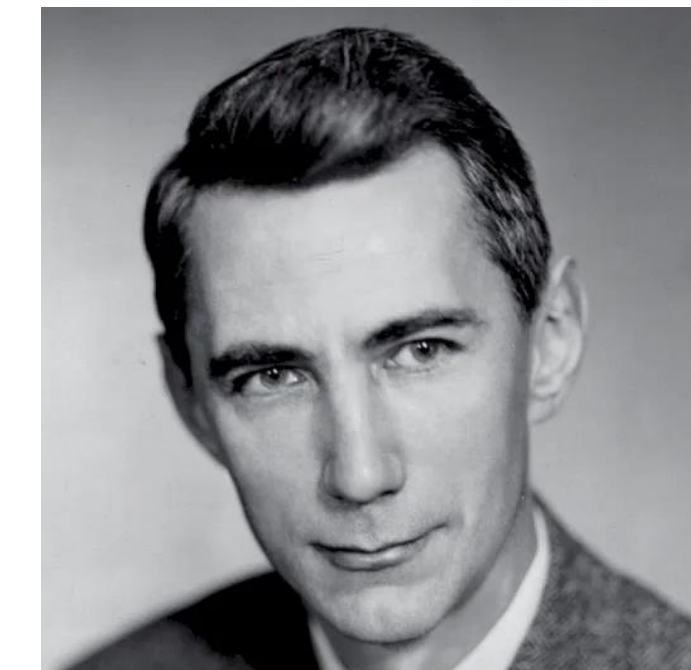
\includegraphics[width=75.60mm,height=184.14mm]{../../images/llm/page_052_img_01.png}%
\end{textblock*}

\end{document}
